\documentclass[12pt,a4paper]{article}
\usepackage[utf8]{inputenc}
\usepackage[francais]{babel}
\usepackage[T1]{fontenc}
\usepackage{amsmath}
\usepackage{amsfonts}
\usepackage{amssymb}
\usepackage{graphicx}
\usepackage[top=3cm, bottom=3cm, left=3cm, right=3cm]{geometry}

\usepackage{verbatim}

\title{Programmation Logique : Prolog}
\author{Valentin NOEL et Romain Pascual}

\begin{document}
\maketitle

\section{Problème 1 : Traversées de rivière}
Les problèmes des traversée de rivière supposent généralement que l'on doit faire passer des individus d'un côté à l'autre de la rivière en ayant un nombre limité de personnage sur le bateau tout en interdisant à certains personnages de rester ensemble d'un même côté de la rivière.

Ici le problème est le suivant : "Lulu doit faire passer le chou, la chèvre et le loup de l'autre côté de la rivière et il n'a qu'une place sur son bateau. Si la chèvre et le chou sont ensemble sur une rive quand Lulu s'éloigne, la chèvre mange le chou. Et si le loup et la chèvre sont ensemble quand Lulu s'éloigne, le loup mange la chèvre."

On cherche à modéliser le problème en Prolog. La solution est donnée dans le fichier "rivière.pl"

La modélisation est la suivante : on utilise un tuple $(Lulu, Chou, Chevre, Loup)$ de booléens tel que chaque variable vaut $0$ si le personnage est du premier côté de la rivière et $1$ s'il est du second. On cherche donc à transformer le tuple $(0,0,0,0,)$ en $(1,1,1,1)$. Pour cela on commence par définir les états interdits (le loup et la chèvre d'un même côté ou encore la chèvre et le chou du même côté). Ensuite on modélise les déplacements possibles : déplacement du chou, de la chèvre, du loup ou de Lulu en interdisant les déplacements qui conduisent à un état interdit.

On cherche ensuite la solution à l'aide d'un parcours en largeur implémenté par des listes.

Le problème est finalement résolu par analogie avec une réflexion sur les graphes où les nœuds représentent les différents états licites et les arcs les déplacements du bateau. La "meilleure" solution est alors obtenue à l'aide d'un parcours en largeur du graphe. Le code du parcours en largeur à été trouvé sur internet et adapté à la situation.

Pour exécuter le code, il suffit d'utiliser la commande \texttt{solution} ou la commande \texttt{solution\_ecrite} dans Prolog après avoir chargé le fichier "rivière.pl". Dans le premier cas, on obtient la liste des situations depuis celle ou tout le monde est sur la première berge jusqu'à celle où tout le monde est sur la seconde berge. Avec la deuxième commande, on obtient la liste écrite des déplacements de Lulu, comme le montre la sortie ci-dessous :

\begin{center}
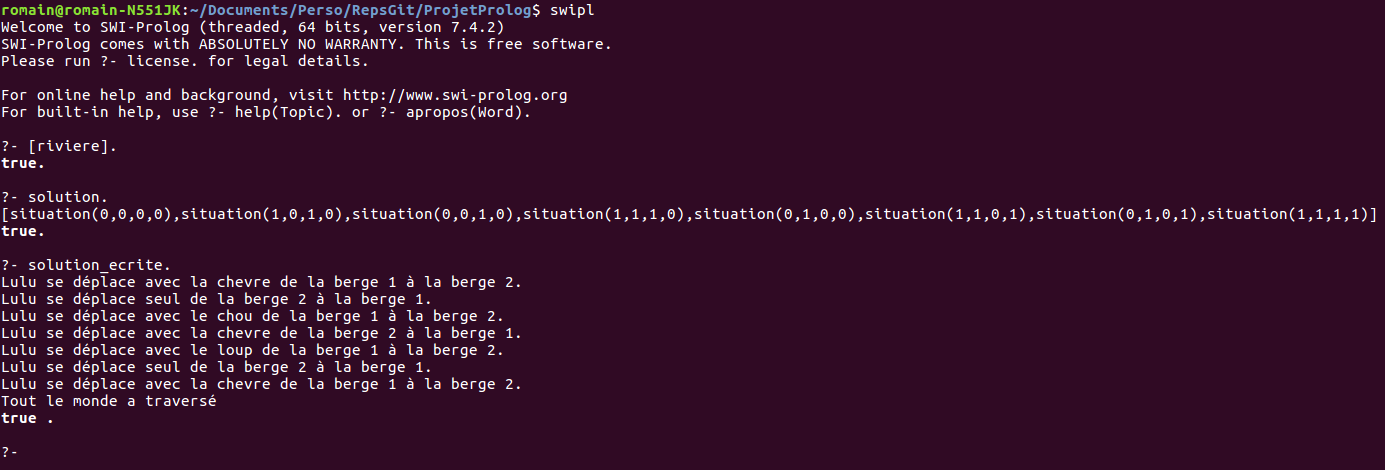
\includegraphics[width = 350pt]{SolutionRiviere.png}
\end{center}


\section{Problème 2 : Le compte est bon}
"Le compte est bon est un jeu (télévisé) qui consiste à trouver une combinaison arithmétique de nombres afin d'obtenir un certain total."

Ici on suppose une entrée avec six nombres $(n_i)_{1 \leqslant i \leqslant 6}$ et un objectif $N$ compris strictement entre $100$ et $1000$. Par ailleurs les nombres $n_i$ sont à choisir parmi $1,2,3,4,5,6,7,8,9,10,25,50,75,100$.

Par exemple, avec le tirage $1,2,3,4,5,6$ et l'objectif $N = 150$, une combinaison gagnante est 

\[ (3*(1 + 2))- 4)*5*6 = 150 \]

Entre deux combinaisons gagnantes, celle qui utilise le moins de nombres sera préférée.

L'implémentation nécessite en premier lieu un certain nombre de prédicats pour pouvoir manipuler les listes (sélection d'un élément, calcul de la longueur, etc.). Le compte est bon est modélisé comme une liste d'opération arithmétiques, on extrait deux nombres, sur lesquels on applique une opération arithmétique ($+$, $-$, $*$ ou *$/$). Le résultat est alors rajouté à la liste des nombres. On obtient ainsi tous les résultats possibles à partir de l'ensemble de départ. Il suffit alors de s'arrêter lorsque l'on a construit l'objectif recherché. Pour obtenir la "meilleure" solution, c'est-à-dire celle utilisant le moins d'opération possibles, on se contente d'énumérer toutes les solutions et d'en choisir une parmi celles ayant le moins d'opérations. Par ailleurs, un certains nombres de prédicats sont utilisés pour vérifier que les contraintes sur les nombres utilisés et sur l'objectif sont remplis. Enfin, on trouvera des prédicats permettant une mise en forme minimale des solutions.
Dans le cas d'une solution approchée, celle si est construite en testant tous les objectifs, en s'éloignant progressivement dans les deux directions.

Le code se trouve dans le fichier "compteEstBon.pl". Pour l'exécuter, il suffit d'appeler la commande \texttt{solution($+$Liste, $+$Nombre)} avec pour paramètres les nombres que l'on peut utiliser et l'objectif à atteindre pour obtenir l'ensemble des solutions possibles. On utilisera la commande \texttt{meilleure\_solution($+$Liste, $+$Nombre)} pour afficher une meilleure solution (en nombre d'opérations). Enfin la commande \texttt{meilleure\_solution\_approchee($+$Nombres, $+$But, $+$Erreur\_toleree)} permet de chercher la meilleure solution approchée restant entre $100$ et $1000$ (exclus) avec pour borne supérieure de l'erreur la valeur de \texttt{Erreur\_toleree}.

Notons que le grand nombre de cas à tester peut causer un certain délais avant d'obtenir le résultat, comme on peut le voir sur les captures d'écran ci-dessous où la valeur $C$ représente le temps d'exécution du code en secondes. 

\begin{center}
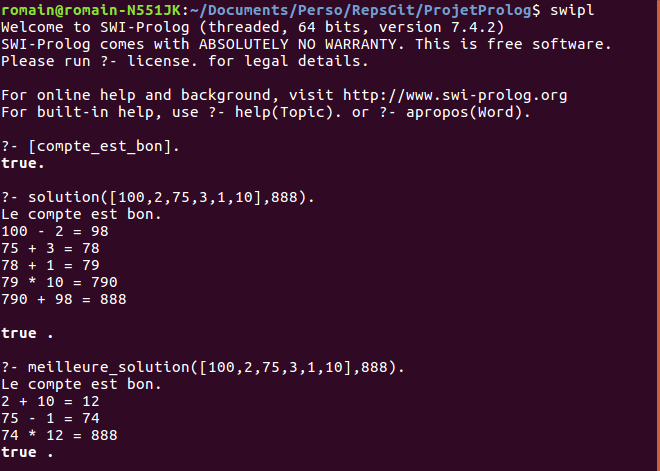
\includegraphics[width = 400pt]{SolutionCompteEstBon1.png}
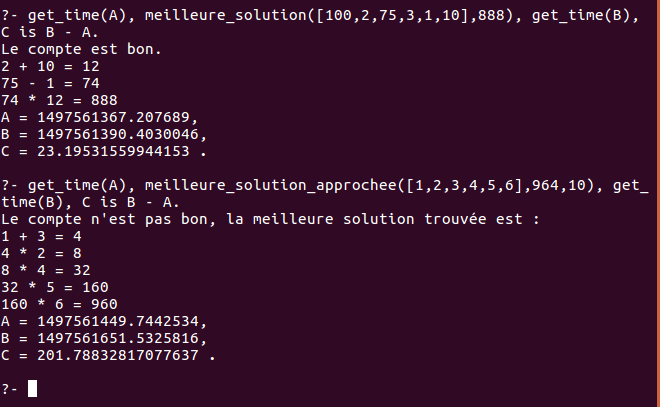
\includegraphics[width = 400pt]{SolutionCompteEstBon2.png}
\end{center}


\section{Problème 3 : Logique propositionnelle}
\subsection{Algorithme DPLL}
Il s'agit d'implémenter un prédicat qui teste la satisfiabilité d'une formule booléenne $\phi$ en appliquant l'algorithme DPLL. On suppose ici que la formule est déjà mise sous forme normale conjonctive. La formule est alors un ensemble de clause et chaque clause est une disjonction de littéraux.  Une clause est alors implémentée sous la forme d'une liste de littéraux et une formule sous la forme d'une liste de liste. Ici on oblige les variables à être représentées avec des entiers naturels. Les littéraux sont alors simplement représentés avec les entiers relatifs : un entier positif représente un variable et un entier négatif la négation de cette variable.

Après avoir défini un certain nombres de prédicats pour manipuler les listes, on implémente des prédicats pour manipuler les littéraux, les clauses et les formules (trouver les littéraux dans une formule, supprimer des littéraux dans une clause ou dans une formule, obtenir la liste des variables d'une formule, etc).

Il s'agit alors de définir les prédicats propres à la résolution avec l'algorithme DPLL :
\begin{itemize}
\item le prédicat \texttt{get\_unitaire} permet de trouver dans une formule sous forme normale conjonctive la liste des littéraux présents dans des clauses unitaires.
\item le prédicat \texttt{get\_polarisation\_positive} permet de trouver dans une formule sous forme normale conjonctive la liste des littéraux possédant uniquement une polarisation positive.
\item le prédicat \texttt{get\_polarisation\_negative} permet de trouver dans une formule sous forme normale conjonctive la liste des littéraux possédant uniquement une polarisation négative.
\end{itemize}

\paragraph{Algorithme} L'algorithme est implémenté de la manière suivante :
\begin{itemize}
\item on cherche les littéraux dans des clauses unitaires, on les modifie les différentes clauses de la formule en fonction de si la valuation des littéraux mis en évidence les valide ou non, puis on résout par DPLL la nouvelle formule ;
\item on cherche les littéraux de valuation uniquement positive, on les modifie les différentes clauses de la formule en fonction de si la valuation des littéraux mis en évidence les valide ou non, puis on résout par DPLL la nouvelle formule ;
\item on cherche les littéraux de valuation uniquement négative, on les modifie les différentes clauses de la formule en fonction de si la valuation des littéraux mis en évidence les valide ou non, puis on résout par DPLL la nouvelle formule ;
\item sinon on prend la variable en tête de liste et on essaie de lui affecter la valeur $true$, on les modifie les différentes clauses de la formule en fonction de si cette valuation les valide ou non, puis on résout par DPLL la nouvelle formule ;
\item lors du backtracking, on prend la variable en tête de liste et on essaie de lui affecter la valeur $false$, on les modifie les différentes clauses de la formule en fonction de si cette valuation les valide ou non, puis on résout par DPLL la nouvelle formule ;
\end{itemize}

Dans un soucis de simplification, on évalue toutes les variables non significatives (c'est-à-dire les variables auxquelles on peut associer $true$ ou $false$ dans modifier la satisfiabilité de la formule) à $true$.


Le code se trouve dans le fichier "dpll.pl", la commande \texttt{solution(+Fnc)} permet d'obtenir une valuation de la formule Fnc décrite comme une liste de liste d'entiers relatifs, comme le montre la capture d'écran ci-dessous :

\begin{center}
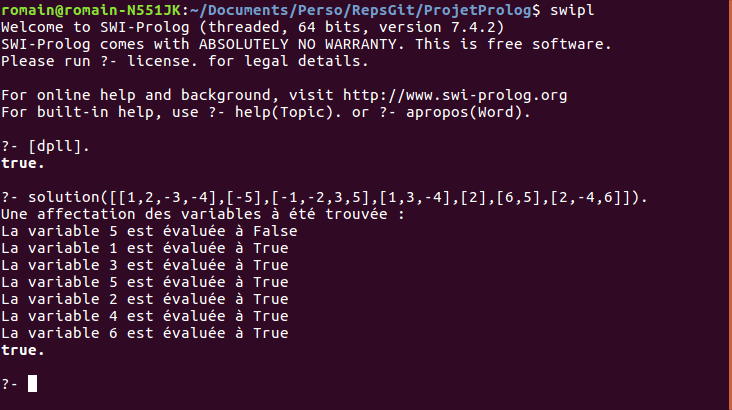
\includegraphics[width = 400pt]{SolutionDpll.png}
\end{center}

Par ailleurs, un prédicat \texttt{temp(+Fnc)} permet d'évaluer le temps d'exécution de la résolution. La figure ci-dessous montre la résolution d'une formule sous forme normale conjonctive issue d'un picross.

\begin{center}
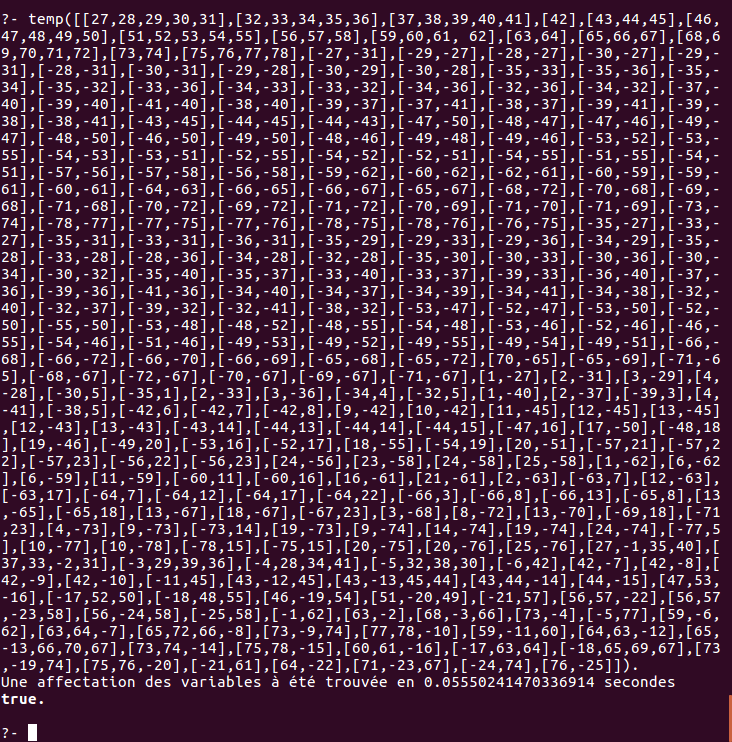
\includegraphics[width = 400pt]{TempDpll.png}
\end{center}

\subsection{Méthode des Tableaux}
Il s'agit d'implémenter un prédicat qui étant donnée une formule $\phi$ indique si $\phi$ est prouvable par la méthode des tableaux (i.e s'il existe un tableau à partir de la négation de $\phi$ dont toutes les branches sont closes). Les tableaux sont manipulés comme des arbres.
\end{document}